\section[Backgroud on quantum metrology]
{Background on quantum metrology}
\thiswatermark{\put(1,-241){\color{l-grey}\rule{84pt}{48pt}}
\put(84,-241){\color{grey}\rule{410pt}{48pt}}}


\quotes{Roger J. Barlow}{In the real world, doing real experiments, statistics began to matter}

\vspace{0pt}
\lettrine[lines=2, findent=3pt,nindent=0pt]{I}{n} this chapter, we will study the basics of quantum metrology, which stands for the study of metrology enhanced by quantum phenomena.
First of all, metrology, as the science of measuring, has played an essential role in the development of science and technology.
Metrology studies several aspects of the estimation process, for example, which strategy to follow in order to improve the precision of the estimation.
Metrology also covers all intermediate processes, from the design aspects of a precise measuring device, to the most basic mathematical concepts that arise from the formulation of the different problems, which lead at the end to a more complete picture of what metrology is.

Historically, with the discovery of quantum theory and the subsequent development of quantum mechanics, new opportunities emerged for advances in metrology in the early decades of the twentieth century.
Later in the last decades of the twentieth century, together with the arrival of concepts like \emph{qubit} and \emph{quantum cryptography}, quantum theory embraced the so-called quantum information theory, which merges the notions of theory of information and computer science with quantum mechanics.
Pushed by the developments of quantum technologies, quantum information attracted much attention from the scientific community.
Moreover, those emerging fields rapidly became into very interesting interdisciplinary playgrounds of science with many scientists as well as resources involved.

At this point, we want to mention that the role of entanglement, an exclusive feature of quantum mechanics which cannot be described using classical probabilistic theories, is essential in this context.
Said this, entanglement is also at the center of the theory of quantum metrology.
Throughout the thesis we will focus mainly on the achievable precision for different systems and schemes.

On the other hand, another very important field of science must be mentioned.
We are talking about statistics, without which many descriptions of the actual and past physical findings would lack the rigorous interpretation needed.
It basically helps to analyze raw data to make it readable from the human perspective.

This chapter is organized as follows.
In Section~\ref{sec:bg-statistics-and-stimation}, we introduce the basic concepts of statistics and estimation theory at the same time we go deeper in the concepts invoked in this thesis.
In Section~\ref{sec:bg-quantum-mechanics-for-metrology}, we present the necessary tools of quantum mechanics used throughout the text.
Finally in Section~\ref{sec:bg-quantum-metrology}, we arrive at the main set of tools used in the quantum metrology framework and by extension in the present work.

\subsection{Background on statistics and the theory of estimation}
\label{sec:bg-statistics-and-stimation}

In this section, we will enumerate the basic concepts of statistics as well as the estimation process.
As we said, the main mathematical tools used by metrology belong to statistics.
Moreover, we are especially interested in estimation theory which shows how to properly estimate some quantity based on some data sample.
The data can be from a set of different heights of a, let us say, basketball team, to the outcomes of a coin toss, or even the wavelength of photons coming out of some radioactive sample.
The aim of this section is to give the reader sufficient material to follow this thesis and make it comprehensible since the beginning\footnote{
For a more detailed material, see Refs.~\citep{Riley2006, Barlow1989}}.

\subsubsection{Probability, data samples, average and variance}

The probability indicates the relative chance of an event to happen.
For instance, if there is a box with ten red balls and five blue balls, considering that the balls of the same color are indistinguishable and that we extract one randomly, we have $\frac{5}{10+5}=\frac{1}{3}$ of probability to obtain a blue ball and $\frac{2}{3}$ to obtain a red ball.
The reader may notice many properties a probability should have, such as that the probability of any event to happen is always given by a number in between zero and one.

When someone has a data sample at hand, it might come from diverse sources and might be represented using multiple forms such as numbers or words (for instance, a table of names of people).
The first thing one tries to accomplish is to analyze the data to extract the relevant properties from it.
A data sample always come from a population sample, i.e., the data sample might not be complete (one could lose some in the process, or the population might be huge in comparison with what one can handle), or might carry some error (a measuring device always has an error when estimating a continuous magnitude, e.g., the height of people), or both at the same time.
Hence, the data sample comes attached with a probability for each data element.
In the subsequent paragraphs, we will describe these relations between the data samples and probabilities and we will enumerate the most useful properties and formulas.

First of all, we will explain our notation which follows mainly the one used in Reference~\citep{Riley2006}.
A probability function gives the probability of an event $x$ to happen when measuring some random variable $X$, and it is denoted by $\prob(X=x)$.
Second, due to the random nature of the measurements, the $N$ elements of a data sample are considered outputs of $N$ different random variables with their corresponding $N$ values $\{X_i=x_i\}_{i=1}^N$, or $\bs{X}=\bs{x}$ for short.
The joint probability of those random variables is in general not separable.
This is due to the fact that the data sample elements could depend on the rest of outcomes or some other more complex relation that makes the most general case to be not separable from the probabilistic point of view.
Therefore we define the probability distribution function (PDF) as an $N$ variable function
\be
  \prob(\bs{X}=\bs{x}) \equiv \prob(X_1=x_1,X_2=x_2,\dots,X_N=x_N).
\ee
In the case of separable probabilities, this is written as
\be
  \label{eq:bg-separable-likelyhood}
  \prob(\bs{X}=\bs{x}) = \prod_{i=1}^N\prob(X_i=x_i)
\ee
which is the case in many relevant situations.

When some indirect property of the system is defined as a function that depends on the measured random variables, the result is also a new random variable with another assigned PDF.
For example, we measure the position of a body at some moment.
If the system was at rest at the origin when $t=0$ and assuming that the acceleration is constant, then from the measured final position one could infer the value of the acceleration by using $A=2X/t^2$, where $X$ denotes the final position at instant $t$ and $A$ the acceleration.
If $X$ is a random variable, which is the general case when measuring the position of some physical system, then the probability assigned for $A$ is computed by
\be
  \prob(A=a) = \left.\frac{\text{d}X}{\text{d}A}\right|_{A=a}\prob(X=x)=\frac{2}{t^2}\prob(X=x).
\ee
In general, for the multiple random variable, we must require the following identity
\be
  |\prob(\bs{X}=\bs{x})\,\text{d}x_1\text{d}x_2\dots\text{d}x_N|=|\prob(\bs{Y}=\bs{y})\,\text{d}y_1\text{d}y_2\dots\text{d}y_N|,
\ee
for any set of random variables.
This leads to some interesting formulas we will discuss later.

We now stick to the simplest case in which the data is a collection of values of the same random variable describing the same physical one-dimensional data population.
Moreover, if the probabilities are independent from each other, the PDF takes the form of Eq.~\eqref{eq:bg-separable-likelyhood}.
Some definitions reasonable to mention in this thesis arise for those kind of data samples: the average, variance, moments and central moments.
The arithmetic average (there are other types of average one can find in the textbooks) is computed by
\be
  \overline{x}=\frac{1}{N}\sum x_i.
\ee
The variance is related to the spread of the data and computed by
\be
  \sigma^2=\frac{1}{N}\sum (x_i-\overline{x})^2,
\ee
where $\sigma$ is the standard deviation.
Different moments are computed by $\overline{x^r}=\frac{1}{N}\sum x_i^r$ while central moments, i.e., statistical moments that are invariant under the translation of the system, are of the form of $c_r=\frac{1}{N}\sum (x_i-\overline{x})^r$.
Note that the variance is the second central moment of the data samples.
For completeness, when each element of the data consists of more than a single number, e.g., $(x_i,y_i)$ where $x_i$ could be the velocity and $y_i$ the acceleration in a experiment to estimate the friction caused by a fluid, the co-variance between two data kinds is obtained by
\be
  V_{X,Y} = \frac{1}{N}\sum_{i=1}^N (x_i-\overline{x})(y_i-\overline{y}).
\ee
Note that we grouped the elements of the data sample into pairs while kept distinctions between both kinds $X$ and $Y$.

We will try to keep this distinction between data sample and data population as clear as possible.
The data population is represented in most cases by the probability distribution function.
In general, the mean values of any function $g(x)$ over the data sample are denoted with a bar over a lowercase variable, e.g., $\overline{x^r}$ for the $r$-th moment over the data sample or $\overline{g(x)}$ for the average of $g(x)$ itself.
On the other hand, the mean values of any function applied to the data population $g(X)$ is denoted following some textbooks by $\text{E}[g(X)]$, e.g., the $r$-th moment over the data population is $\text{E}[X^r]$.
One clearly may distinguish two cases when we talk about data populations.
While the data sample is always consist of discrete data elements, the data population can be represented by a PDF for discrete values or it can be represented by a PDF for values that can take any real number.
For completeness, here are expressed the two definitions for the mean value over the data population, i.e., represented by a PDF, of a function $g(\bs{X})$ by
\be
  \label{eq:bg-expectation-value-of-any}
  \text{E}[g(\bs{X})] = \lcor
  \begin{split}
    &\int g(\bs{x}) \prob(\bs{X}=\bs{x})\,\text{d}^N \bs{x},\\
    &\sum_{i,j,\dots} g(\bs{x}) \prob(\bs{X}=\bs{x}).
  \end{split}
  \right.
\ee
At this point, one more straight forward definition needs our attention, the variance of a function $g(X)$ over the data population is denoted by $\text{V}[g(X)] \equiv \text{E}[g(X)^2] - \text{E}[g(X)]^2$.

\subsubsection{Frecuentist vs. bayesian approach}

\subsubsection{Estimators and Fisher information}
\label{sec:bg-estimators}

Let us suppose that the data sample has encoded some desired parameters $\bs{a}\equiv(a_1,a_2,\dots)$.
The underlying probability, in general also unknown, may be conditioned by the real values of the parameters $\bs{a}$.
The probability of the data sample is therefore written as
\be
  \prob(\bs{X}=\bs{x}|\bs{a}),
\ee
where "$|\bs{a}$" indicates its dependency on these parameters.
At this point, note that an estimate of one of the desired parameters must be based on the data sample elements.
A function of this type is called the \emph{estimator} and it is connected with the PDF of the data population.
Hence as mentioned before, an estimator of $a$, one of the unknown parameters, is denoted by $\hat{a}$ and the PDF associated to it is computed from the PDF of the data population as
\be
  \prob(\hat{a}|\bs{a})\,\text{d}\hat{a} = \prob(\bs{x}|\bs{a})\,\text{d}x_1\text{d}x_2\dots\text{d}x_N.
\ee
For short, we have omitted writing "$\bs{X}=$", thus the conditional joint probability of $N$ random variables $\bs{X}$ is written simply as $\prob(\bs{x}|\bs{a})$.

As we said, an estimator is defined to be a function of the data sample.
For example, one of such estimators is the estimator of the mean value of the population, in general unknown.
The mean value of the data population, which in general we do not have access to, is denoted usually by $\mu$.
Note that $\mu$ is in general different from the mean value of the data sample $\overline{x}$.
A valid estimator for the mean value $\mu$ would be the mean itself of the data sample, i.e., $\hat{\mu}=\overline{x}$.

An important notion of an estimator is its \emph{efficiency}.
The smaller the variance of the estimator the more efficient it is.
Remember than an estimator is considered a random variable so it must have a variance when our knowledge about the population is incomplete, i.e., when we estimate it from the data sample.

Focusing into what it is more interesting for of this thesis, an estimator of any kind has a theoretical lower bound for its variance.
For the proof of the previous statement, which we will compute for continuous random variables without losing of generality, we start with the normalization formula of a given PDF
\be
  \int \prob(\bs{x}|\bs{a})\,\text{d}^N\bs{x} = 1.
\ee
Next, we compute the partial derivative over $a$, one of any of the unknown parameters, such that
\be
  \label{eq:bg-expectation-value-of-logarithm}
  \int \partial_a\prob(\bs{x}|\bs{a})\,\text{d}^N\bs{x} = \int \partial_a\big(\ln  \prob(\bs{x}|\bs{a})\big) \prob(\bs{x}|\bs{a}) \,\text{d}^N\bs{x} = 0,
\ee
where for the second equality we used the identity for logarithmic derivatives.
From Eq.~\eqref{eq:bg-expectation-value-of-any}, it turns out that the Eq.~\eqref{eq:bg-expectation-value-of-logarithm} is the expectation value of $\partial_a(\ln\prob)$.
Finally, if we have an \emph{unbiased} estimator, i.e., an estimator for which the expectation value $\text{E}[\hat{a}]$ coincides with true value $a$ of the unknown parameter, the partial differentiation of $\text{E}[\hat{a}]$ over $a$ must be equal to one.
Therefore, we apply similar identities as in Eq.~\eqref{eq:bg-expectation-value-of-logarithm} to arrive at
\be
  \label{eq:bg-expectation-of-estimator-derivated}
  \begin{split}
    \partial_a\text{E}[\hat{a}] &= \partial_a a
    = \partial_a \int \hat{a} \prob(\bs{x}|\bs{a})\,\text{d}^N\bs{x} \\
    &=  \int \hat{a} \partial_a\prob(\bs{x}|\bs{a})\,\text{d}^N\bs{x} =  \int \hat{a} \partial_a\big(\ln  \prob(\bs{x}|\bs{a})\big) \prob(\bs{x}|\bs{a}) \,\text{d}^N\bs{x} = 1,
  \end{split}
\ee
where we have used the definition of the expectation value for continuous variables Eq.~\eqref{eq:bg-expectation-value-of-any} and we use the fact that the estimator is not a function of the parameter $a$.

At this point, we invoke the Schwartz inequality for two real multidimensional functions $g(\bs{x})$ and $h(\bs{x})$ such that $(\int g h \,\text{d}^N\bs{x})^2\leq (\int g^2 \,\text{d}^N\bs{x}) (\int h^2 \,\text{d}^N\bs{x})$.
With this, we can follow step by step the following recipe to obtain a lower bound for the variance of a general estimator.
First the definition of the variance over the data population looks like
\be
  V[\hat{a}] = E[(\hat{a}-a)^2] = \int (\hat{a} - a)^2\prob(\bs{x}|\bs{a})\,\text{d}^N\bs{x},
\ee
remember that the estimator is assumed to be unbiased.
Second, subtracting $a$ times Eq.~\eqref{eq:bg-expectation-value-of-logarithm} to Eq.~\eqref{eq:bg-expectation-of-estimator-derivated} the following holds,
\be
  \int (\hat{a}-a)\partial_a\big(\ln  \prob(\bs{x}|\bs{a})\big) \prob(\bs{x}|\bs{a})\,\text{d}^N\bs{x} = 1
\ee
because $a$ is not a function of $\bs{x}$.
Hence, using the Schwartz inequality we can write
\be
  \label{eq:bg-classical-cr-bound-and-fi}
  \text{V}[\hat{a}] = \int (\hat{a} - a)^2\prob(\bs{x}|\bs{a})\,\text{d}^N\bs{x} \geq \frac{1}{\int \lcua\partial_a\big(\ln \prob (\bs{x}|\bs{a}) \big)\rcua^2 \prob (\bs{x}|\bs{a})\,\text{d}^N\bs{x}},
\ee
which is also known as the Cram\'er-Rao bound or the Fisher inequality.
The denominator on the right hand-side is called generally the Fisher information (FI) or simply information.

With this review of the most interesting properties of "classical" metrology, from the point of view of this thesis, we conclude this section.
In the next section, we will discuss some properties of the quantum mechanics and then we will follow with another section which presents the basis of quantum metrology.

\subsection{Quantum mechanics from metrology perspective}
\label{sec:bg-quantum-mechanics-for-metrology}

The ubiquitous probabilistic nature of quantum mechanics makes us to work with probabilities on a regular basis.
Moreover, if one studies fields connected to experiments or some short of physical realizations, this probabilistic nature of quantum mechanics becomes even more visible.
On the other hand, exotic features such as entanglement arise from quantum mechanics, which is directly connected with the probabilistic notions explained before.
The present section is intended to describe quantum systems from the point of view of metrology.

\subsubsection{The quantum state, multiparticle state, entanglement}
\label{sec:bg-the-quantu-state}

A formal mathematical description of the quantum state is given next.
This also allows us to introduce some notation used throughout the thesis.
A \emph{state} in quantum mechanics lives on a Hilbert space, $\mathcal{H}$.
The state, $\rho$, has the following properties:
\begin{enumerate}
  \item
  It is Hermitian, so it is invariant under the complex transposition, $\rho=\rho^\dagger$ and all its eigenvalues are real.
  \item Its trace is equal to one, $\tr(\rho)=1$.
  \item It is positive semi-definite, i.e, all its eigenvalues are bigger or equal to zero, $\rho=\sum_{\lambda}p_\lambda \Pi_\lambda$ where $p_\lambda\geq 0$ and $\Pi_\lambda\equiv\ketbra{\lambda}{\lambda}$ is the projector of the eigenstate $\ket{\lambda}$, a vector state satisfying the following eigenvalue equation $\rho\ket{\lambda}=p_{lambda}\ket{\lambda}$.
  From (ii), it follows that $\sum_\lambda p_\lambda = 1$.
  \item If all $p_\lambda$ are zero except one, the state is called a pure state and is equivalent to the projector of such eigenstate $\rho=\Pi_\lambda=\ketbra{\lambda}{\lambda}$.
  \item Using the properties (iii) and (iV), it follows that the quantum states form a convex set where the extreme must be pure states.
  \item An expectation value of an observable $\mathcal{O}$ is computed as $\expect{\mathcal{O}}=\tr(\mathcal{O}\rho)$.
  To make a connection with the previous section, the state represents the so-called data population, hence using the notation in Sec.~\ref{sec:bg-statistics-and-stimation},  $\expect{\mathcal{O}}\equiv\text{E}[\mathcal{O}]$.
\end{enumerate}

The composite system of $N$ different parties live in the Hilbert space $\mathcal{H} = \mathcal{H}^{(1)}\otimes\mathcal{H}^{(2)}\otimes\cdots\otimes\mathcal{H}^{(N)}$ or $\mathcal{H} = \bigotimes_{i=1}^N\mathcal{H}^{(i)}$ for short, where $\otimes$ stands for tensor product.
For instance, this composite Hilbert space could be used to represent a many-particle system, in this case $N$ particles.
A \emph{separable} state in this Hilbert space can be written as
\be
  \label{eq:bg-separable-state-definition}
  \rho_{\text{sep}} = \sum_{i}p_i\rho_i^{(1)}\otimes\rho_i^{(2)}\otimes\cdots\otimes\rho_i^{(N)},
\ee
where $p_i$ are convex weights that add up to one and are equal to or bigger than zero.
If a state cannot be written like Eq.~\eqref{eq:bg-separable-state-definition}, the state is said to be \emph{entangled}.
We mention it as a formal description of the entanglement \citep{Guehne2009, Luis2004}.
One may note at this moment, that relaxing the requirements of Eq.~\eqref{eq:bg-separable-state-definition}, one can lead to different classifications of the states.
Concepts like genuine multipartite entanglement, $k$-producible states, or entanglement depth, among others, arose from weaker constraints than Eq.~\eqref{eq:bg-separable-state-definition} \citep{Guehne2009, Luis2004}.

It is important to describe one of such classifications in order to characterize the different levels or multipartite entanglement followed in this work.
We call a state $k$-producible, if it \emph{can} be written as a mixture of the tensor product of different multipartite states with at most $k$ parties in each,
\be
  \label{eq:bg-k-producible-estate}
  \rho_{k\text{-pro}} = \sum_i p_i\rho^{(\alpha,\dots,\beta)}_i \otimes \rho^{(\gamma,\dots,\delta)}_i\otimes \dots,
\ee
where superscript indexes between parenthesis go from 1 to $N$ and denote to which parties belong to the state, and where each index appears once in each sum element.
For instance a separable state like Eq.~\eqref{eq:bg-separable-state-definition} is 1-producible as well as $N$-producible.
If a state cannot be written as $k$-producible, then it must be $(k+1)$-entangled.
This defines the entanglement depth, see Figure~\ref{fig:bg-separability-k-producibility-circle}.
\begin{figure}[htp]
  \centering
  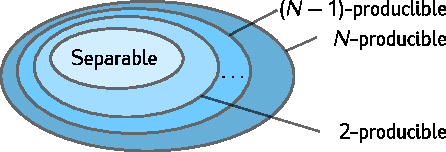
\includegraphics[scale=1.2]{img/BG_separability_k_producibility_circle.pdf}
  \caption[Diagram for $k$-producibility sets]{$k$-producible set of states contains $k-1$-producible states. Based on the Eq.~\eqref{eq:bg-k-producible-estate}, one can argue that a state that cannot be written as $k$-producible must be $k+1$-entangled or equivalently has $k+1$ entanglement depth. A separable state can always be written as 1-producible which on the other hand is its original definition.}
  \label{fig:bg-separability-k-producibility-circle}
\end{figure}
Later on, these concepts of entanglement and entanglement depth will arise naturally on the metrological framework \citep{Toth2014}.

\subsubsection{Angular momentum operators for multipartite systems}
\label{sec:bg-angular-momentum-operators}

Besides those concepts, we present a set of operators that will appear many times in all chapters, namely the angular momentum operators.
Again these definitions allow us to introduce much of the notation used on this book.
For a single party with discrete $d$ levels, and therefore with a spin $j=(d-1)/2$, the eigenvalue equation for the angular momentum projection operators are
\be
  j_l^{(n)}\ket{m}_l^{(n)} = m \ket{m}_l^{(n)}
\ee
for $m=-j,\dots,+j$, where $l=x,y,z$.
It is usual to omit the subscript of $\ket{m}_l^{(n)}$ when $l=z$ because it is the preferred direction for many authors and the superscript ($n$) can also be omitted when the single-particle states are given in an ordered form to build a multiparticle state, i.e., $\ket{\psi} = \ket{m_1}\ket{m_2}\dots\ket{m_n}$ where we also omitted writing the tensor product operator $\otimes$ in between single-particle states.
In many cases, it is also usual to merge all into a single ket state $\ket{\psi}=\ket{m_1 m_2 \dots m_N}$ for simplicity\footnote{
This notation is normally used in many-body quantum mechanics, see Refs.~\citep{Cohen-Tannoudji1977, Sakurai2014}.}.

The square of the total angular momentum, $\bs{j}^2=j_x^2+j_y^2+j_z^2$, for a single party $(n)$ acts on any state simply as
\be
  (\bs{j}^2)^{(n)}\rho=j_n(j_n+1)\rho,
\ee
where state must be defined in a Hilbert space containing $\mathcal{H}^{(n)}$, the Hilbert space of $n^{\text{th}}$ particle and where $j_n$ is the spin number of such a particle.
Note that in order to distinguish the spin number $j_n$ and the operators $j_l^{(n)}$ we may use the fact that the operators are attached to a Hilbert space with a superscript or even we can use a "hatted" notation to denote which of them is an operator like $\hat{j_l}$ and which is not.

The collective angular momentum projection operators $J_l$ are defined as the sum of their respective single-party spin operators $j_l^{(n)}$ such that they are extended to the remaining of the Hilbert spaces by tensor products of the identity operators defined for the rest of subspaces,
\be
  \label{eq:bg-total-angular-momentum-progection-operators}
  J_l = \sum_{i=1}^N \mtxid^{(1,\dots, i-1)} \otimes j_l^{(i)} \otimes \mtxid^{(i+1,\dots,N)} \equiv \sum_{i=1}^N j_l^{(i)},
\ee
where $\mtxid$ stand for the identity operator and the last formula is the most used since it is easy to note that the single-party operator must be extended in order to sum the correctly.
On the other hand, note that the squares of the different projections of total angular momentum are not equal to the sum of the square angular momentum projections of each of the parties.
Thus we obtain that
\be
  J_l^2 = \sum_{i,j}^N j_l^{(i)} j_l^{(j)} = \sum_{i=1}^N (j_l^2)^{(i)}+\sum_{i\neq j}^N j_l^{(i)} j_l^{(j)}.
\ee
Therefore, neither square of the total angular momentum is the sum of the square of all single-party angular momenta but
\be
  \bs{J}^2 = \sum_{i}^N \bs{j}^{(i)} + \sum_{l=x,y,z}\sum_{i\neq j}^N j_l^{(i)} j_l^{(j)},
\ee
where we separated the sum into two parts, the first one corresponds to the sum of all single party angular momentum projections squared and the second corresponds to the product of angular momentum projection operators of two distinct subsystems summed for all $l=x,y,z$.
Many more combinations of these single-party operators may arise in different contexts.
In the Appendix~\ref{app:angular-subspaces}, we discuss in more detail the different structures that arise from adding the angular momentum operators, e.g., the symmetric subspace or the singlet subspace.

\subsubsection{Dynamics of quantum systems}

The most basic evolution of the state is represented by unitary evolution operators denoted by $U$ and those are the only ones appearing throughout the thesis.
On the other hand, there are other types of dynamics involving particle loss, entropy changes in the system and open quantum systems in general.
These transformations are governed by master-equations such as the Lindblad equation \citep{Lindblad1976, Nielsen2000, Breuer2002}.

For the understanding of this thesis it is enough to present the unitary evolution operators.
We also restrict ourselves to the case in which the evolution is constant in time, so are in general the Hamiltonians of the metrological setups.
The unitary evolution operators is defined as
\be
  U = \exp(-i \alpha G)=\sum_{n=0}^{\infty} \frac{(-i \alpha G)^n}{n!},
\ee
where we use the matrix exponentiation in the last equality, $G$ represents a Hermitian operator usually called generator and $\alpha$ is the amount of change.
When a constant Hamiltonian $H$ acts on an initial state $\rho$, the state evolves in time as
\be
  \rho(t) = U\rho U^{\dagger} = e^{-i\frac{tH}{\hbar}} \rho e^{+i\frac{tH}{\hbar}}.
\ee
Note that all information we can extract from the system comes in the form of expectation values of different operators at different times, $\expect{\mathcal{O}}(t) = \tr(\mathcal{O}\rho(t))$.
When the state evolves in time but the operators are constant the picture of the system is called the Schrodinger-picture.
Using the cyclic property of the trace, $\tr(ABC) = \tr(CBA)$, the Heisenberg-picture, a dual interpretation of the same physical system in which the state remains the same while the operators evolve in time, emerges.
It is well known that the operators in this picture evolve as $\mathcal{O}(t) = U^{\dagger} \mathcal{O} U$, where $\mathcal{O}$ is the initial operator.
One can check different textbooks of quantum mechanics, just to mention some see Refs.~\citep{Cohen-Tannoudji1977, Sakurai2014}.

\subsection{Quantum metrology}
\label{sec:bg-quantum-metrology}

We summarize important recent advances in quantum metrology.
Simple metrological setups allow for encoding some desired parameter into the state of the system, thus from the readout of the final state one could infer it.
The basic ideas of quantum metrology emerge when one applies the notions of estimation theory to the intrinsic probabilistic nature of quantum mechanics.
Merging the probabilistic features of quantum mechanics and the estimation theory is not trivial.
Nevertheless, with the initial pioneering works of W. K. Wootters, and S. L. Braunstein and C. M. Caves, in 1981 and 1992-1994 respectively \citep{Wootters1981, Braunstein1992, Braunstein1994}, until the works of V. Giovannetti et al, and M. G. Paris, roughly two decades later \citep{Giovannetti2004, Paris2009}, the foundations of quantum metrology were stabilized.
% TD: important citations needed here!!
Later, advanced works in quantum metrology appeared \citep{XXX} together with experimental realizations \citep{Behbood2013, Koschorreck2011, Luecke2011} which raised the interest in this topic.
In this section, we will highlight the most important aspects of this field and with this we will conclude this chapter for presenting the background theory in which stands the work developed by the authors.

The most basic scheme for a metrological setup in the present context is the following.
First, a state $\rho$ is prepared followed by a general evolution represented by a mapping $\Lambda_{\theta}$ in which the unknown parameter $\theta$ is imprinted into the state.
Finally, the outgoing state is characterized by some measured quantity $\expect{M}$, which allows to infer the value of the parameter $\theta$.
Figure~\ref{fig:bg-preparation-encoding-estimation} illustrates the main steps of quantum metrology.
\begin{figure}[htp]
  \centering
  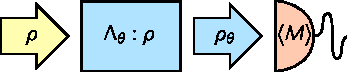
\includegraphics[scale=1.2]{img/BG_preparation_encoding_estimation.pdf}
  \caption[The estimation process in quantum metrology]{Sequence of the different steps for the basics of the estimation process in quantum metrology. First, an input state $\rho$ enters the region in which the unknown parameter $\theta$ is imprinted in it, for the most general case, represented with $\Lambda_{\theta}$. The state with the encoded parameter $\theta$ is measured and $\theta$ must be inferred from the measured quantity $\expect{M}$.}
  \label{fig:bg-preparation-encoding-estimation}
\end{figure}

In the many-particle case, most of the metrology experiments have been done in systems with simple Hamiltonians that do not contain interaction terms.
Such Hamiltonians cannot create entanglement between the particles.
A typical situation is that we rotate our many particle state by some angle and we want to estimate the rotation angle $\theta$.
It has been shown that particles exhibiting quantum correlations, or more precisely, quantum entanglement \citep{Guehne2009, Luis2004}, provide a higher precision than an ensemble with non-entangled particles.
The most important question is how the achievable precision of the angle estimation $\varian{\theta}$ scales with the number of particles.
Very general derivations lead to, at best,
\be
  \label{eq:bg-shot-noise-scaling}
  \varian{\theta}\sim \frac{1}{N}
\ee
for non-entangled particles.
The equation above is called \emph{shot-noise} or standard scaling (SNS), the term originating from the shot-noise in electronic circuits, which is due to the discrete nature of the electric charge.
On the other hand, quantum entanglement makes it possible to reach
\be
  \label{eq:bg-heisenberg-scaling}
  \varian{\theta}\sim \frac{1}{N^2}
\ee
which is called the \emph{Heisenberg} scaling (HS).
Note that if the Hamiltonian of the dynamics has interaction terms, then these bounds can be surpassed \citep{Luis2004, Napolitano2011, Boixo2007, Braun2011, Roy2008, Choi2008, Rey2007}.

It is time to mention that the above calculations have been carried out for an ideal situation.
When an uncorrelated noise is present in the system, it turns out that for large enough particle number the scaling becomes a SNS \citep{Demkowicz-Dobrzanski2012}.
The possible survival of a better scaling under correlated noise, under particular circumstances, or depending on some interpretation of the metrological task, is at the center of attention currently.
All these are strongly connected to the question of whether strong multipartite entanglement can survive in a noisy environment.

Finally, note that often, instead of $\varian{\theta}$ one calculates its inverse, which is large for high precision.
It scales as $\varinv{\theta}\sim N$ for SNS and as $\varinv{\theta}\sim N^2$ for the HS.

\subsubsection{Quantum magnetometry}
\label{sec:bg-quantum-magnetometry}

Without loss of generality, we present in this section the characterization of the precision of one of the simplest metrological tasks, namely the estimation of a homogeneous magnetic field based on the interaction between the system and the field.
In this section, we will mostly study the interaction of a system with a homogeneous field in the $z$-direction.
In the Chapter~\ref{sec:gm}, we will show a different situation in which the magnetic field changes linearly with the position of the system.
With the aim of estimating the strength of the magnetic field, a state is used in order to interact with it, coupling the magnetic moment of the state and the external magnetic field.
Finally, measuring how the state has changed one could in principle infer on the strength of the magnetic field.

In general, we will say that the magnetic moments of the states come exclusively from the spin angular momentum, neglecting any possible contribution from the orbital angular momentum.
This way the physics is simpler.
This is justified in the sense that most of the recent experiments in this context have been carried out with ion-traps, Bose-Einstein condensates (BEC) or at most cold atomic ensembles, which have indeed a negligible orbital angular momentum.

Beside this considerations, the interaction Hamiltonian can be written as
\be
  H = - \bs{\mu} \cdot \bs{B}
\ee
up to some constant factor.
Now in the simplest case we will choose the magnetic field to be pointing to some fixed direction, for instance, the $z$-direction.
So the magnetic field vector can be written as ${B}=B\bs{k}$, where $\bs{k}$ is the unitary vector pointing to the $z$-direction.
This way the estimation problem is much simpler, since one does not need to determine the direction of the magnetic field.

The magnetic moment of the system is proportional to the spin angular momentum, $\bs{\mu}=-\mu_\text{B} g_{\text{s}}\hbar^{-1} \bs{J}$, where $\mu_{\text{B}}$ and $g_{\text{s}}$ are the Bohr magneton and anomalous gyromagnetic factor respectively.
Finally, one can rewrite the interaction Hamiltonian as
\be
  \label{eq:bg-hamiltonian-homogeneous-field}
  H = \gamma B J_z,
\ee
where $\gamma = \mu_\text{B} g_{\text{s}}\hbar^{-1}$ and we have used the fact that $\bs{J}\cdot\bs{k}=J_z$.
Finally, the unitary operator leading the evolution of the system can be written as
\be
  \label{eq:bg-unitary-homogeneous-field}
  U = \exp(-i\theta J_z),
\ee
where the magnetic field strength is encoded into the phase-shift $\theta=-\mu_\text{B} g_\text{s} t B/\hbar$.
Here $\mu_\text{B}$ stands for the Bohr magneton and $g_\text{s}$ for the giro-magnetic constant for the spin angular momentum, and $t$ is the evolution time.

We have to mention as well that for large particle ensembles, typically only collective quantities can be measured in order to characterize the state on different phases of the metrological sequence, see Figure~\ref{fig:bg-preparation-encoding-estimation}.
Such collective quantities are in this case the angular momentum components defined in Eq.~\eqref{eq:bg-total-angular-momentum-progection-operators} and their combinations.
More concretely, we can measure the expectation values of any direction
\be
  \label{eq:bg-total-angular-momentum-projector-arbitrary-direction}
  J_{\bs{n}}:=\sum_{l=x,y,z} n_l J_l,
\ee
where $\bs{n}=(n_x,n_y,n_z)$ is a unit vector describing the direction of the component.

\subsubsection[Metrology with almost polarized states]{Metrology with almost polarized states, including spin-squeezed states}

Let us present one of the basic approaches to calculate the metrological precision of a quantum setup.
In order to estimate the phase-shift $\theta$ we measure the expectation value of a Hermitian operator, which we will denote by $M$ in the following.
If the evolution time is a constant then estimating $\theta$ is equivalent to estimating the magnetic field strength $B$ in Eq.~\eqref{eq:bg-hamiltonian-homogeneous-field}.
The precision of the estimation can be characterized with the error propagation formula as
\be
  \label{eq:bg-error-propagation-formula}
  \varian{\theta} = \frac{\varian{M}}{|\partial_\theta\expect{M}|^2},
\ee
where $\expect{M}$ is the expectation value of the operator $M$, and we used the assumption that $\expect{M}$ is a random variable and that it has a PDF that can relate $\prob(\expect{M}|\theta)$ with a PDF as a function of the estimator $\prob(\hat{\theta}|\theta)$, see the Section~\ref{sec:bg-estimators}, and for a recent review discussing this approach in detail, see Ref.~\citep{Kolodynski2010}.
Thus, the precision of the estimate depends on how sensitive $\expect{M}$ is to the change of $\theta$, and also on how large the variance of $M$ is.
Based on the formula Eq.~\eqref{eq:bg-error-propagation-formula}, one can see that the larger the slope $|\partial_\theta \expect{M}|$, the higher the precision.
On the other hand, the larger the variance $\varian{M}$, the lower the precision.
Figure~\ref{fig:bg-expect-m-evo} helps to interpret the quantities appearing in Eq.~\eqref{eq:bg-error-propagation-formula}.
\begin{figure}[htp]
  \centering
  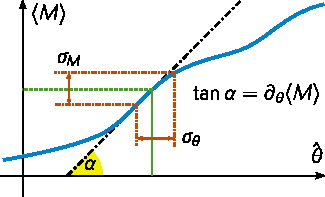
\includegraphics[scale=1.2]{img/BG_expect_m_evo.pdf}
  \caption[Graphical explanation of the error-propagation formula]{(Blue solid) Functional relation between the expectation value $\expect{M}$ and the estimator of the wanted parameter $\hat\theta$.
  (Green dashed) One to one correspondence when the estimator $\hat{\theta}$ is based on $\expect{M}$. (Red dotted) Obtaining the error of the estimate is based on Eq.~\eqref{eq:bg-error-propagation-formula}.
  The slope of the curve at that point, denoted with $\tan\alpha$, directly relates the uncertainty $\sigma_M$ on the measured quantity $\expect{M}$ and the error on the estimation $\sigma_\theta$.}
  \label{fig:bg-expect-m-evo}
\end{figure}

We focus on multi-partite systems of spin-$\frac{1}{2}$ particles, widely known in the field as qubits, for homogeneous magnetometry in order to simplify the discussion.
For this, let us start with an almost polarized state.
The spin vector of the ensemble, originally pointing into the $y$-direction, will be rotated.
The rotation after the evolution is used to estimate the strength of the magnetic field.
A way to measure the rotation suffered by the system is to measure the expectation value $\expect{J_x}$, which is zero at the beginning.

For small angles of $\theta$ and using the Eq.~\eqref{eq:bg-error-propagation-formula} after substituting $M$ by $J_x$, we arrive at
\be
  \label{eq:bg-error-propagation-measuring-jx}
  \varinv{\theta} = \frac{|\partial_\theta \expect{J_x}|^2}{\varian{J_x}},
\ee
for a state almost completely polarized along the $y$-axis.
Next, we have to compute these values for small angles of $\theta$.

To compute them we use the Heisenberg picture of the operator $J_x$, that after applying the unitary operator Eq.~\eqref{eq:bg-unitary-homogeneous-field}, is written as
\be
  J_x(\theta) = U^{i\theta J_z} J_x U^{-i\theta J_z} = \coss{\theta}J_x -  \sins{\theta} J_y,
\ee
where we also introduced a notation for trigonometric functions since they will appear many times in this work, $\coss{x} \rightarrow \cos(x)$, $ \sins{x}\rightarrow\sin(x)$ and $\tans{x}\rightarrow\tan(x)$.
Thus, the square of $J_x$ is simply
\be
  J_x^2(\theta) = \coss{\theta}^2J_x^2 -2 \coss{\theta}\sins{\theta}\{J_x,J_y\}+  \sins{\theta}^2 J_y^2,
\ee
where $\{A,B\}=AB+BA$ is the anti-commutator, since the operators may not commute in general and in this particular case it is not an exception.
Finally we compute the derivative with respect to $\theta$ of $\expect{J_x}$ as
\be
  \partial_{\theta}\expect{J_x}(\theta)=\partial_{\theta}\coss{\theta}\expect{J_x} - \partial_{\theta}\sins{\theta}\expect{J_y} = -\sins{\theta}\expect{J_x}-\coss{\theta}\expect{J_y},
\ee
where we used the linearity of the trace to compute the expectation value and the linearity of the derivative.

Hence, assuming that we are in the small angle limit to compute the Eq.~\eqref{eq:bg-error-propagation-measuring-jx}, we may take the terms proportional to $\sin(\theta)$ as zero.
Therefore, when we measure $\expect{J_x}$ to estimate the angle $\theta$, the precision of the estimation is given by
\be
  \label{eq:bg-error-propagation-measuring-jx-computed}
  \varinv{\theta} = \frac{|\coss{\theta}\expect{J_y}|^2}{\coss{\theta}^2\expect{J_x^2} - (\coss{\theta}\expect{J_x})^2} = \frac{\expect{J_y}^2}{\varian{J_x}}.
\ee

For the state totally polarized along the $y$-axis, the initial expectation values $\expect{J_x}$, $\expect{J_x^2}$ and $\expect{J_y}$ needed to compute the precision are
\be
  \begin{split}
    \expect{J_x}_{\text{tp}}  & = 0,\\
    \expect{J_x^2}_{\text{tp}}  & = \tfrac{N}{4},\\
    \expect{J_y}_{\text{tp}}  & = \tfrac{N}{2}.
  \end{split}
\ee
Thus, we obtain a precision that scales linearly with $N$,
\be
  \varinv{\theta}_{\text{tp}} = \frac{N^2/4}{N/4} = N.
\ee
Note that the totally polarized state is a separable pure state with all particles pointing into the $y$-direction.
We obtained the shot-noise scaling, even with very simple, qualitative arguments

A way of improving the precision is considering that the variances of the angular momentum components are bounded by the Heisenberg uncertainty relation \citep{Kitagawa1993}
\be
  \varian{J_x}\varian{J_z} \geq \frac{1}{4}|\expect{J_y}|.
\ee
Due to decreasing $\varian{J_x}$, our state fulfills
\be
  \varian{J_x}<\frac{1}{2}|\expect{J_y}|,
\ee
where the main spin points along the $y$-axis and for totally polarized states $\varian{J_x}=\frac{1}{2}|\expect{J_y}|$ hold.
Such states are called \emph{spin-squeezed} states \citep{Kitagawa1993, Wineland1994, Sorensen2001, Ma2011} and they can in principal overcome the SNS.

Next, we can ask, what the best possible phase estimation precision is for the metrological task considered in this section.
For that, we have to use the following inequality based on general principles of angular momentum theory
\be
  \label{eq:bg-total-angular-momentum-saturability}
  \expect{J_x^2+J_y^2+J_z^2} \leq \frac{N(N+2)}{4}.
\ee
Note that Eq.~\eqref{eq:bg-total-angular-momentum-saturability} is saturated only by symmetric multiparticle states, see Appendix~\ref{app:angular-subspaces}.
Together with the identity connecting the second moments, variances and expectation values
\be
  \varian{J_l} + \expect{J_l}^2 = \expect{J_l^2},
\ee
Eq.~\eqref{eq:bg-total-angular-momentum-saturability} leads to a bound on the uncertainty in the anti-squeezed direction, in this case $z$-direction, for the variance
\be
  \varian{J_z} \leq \frac{N(N+2)}{4} - \expect{J_y}^2 = \frac{N}{2} + \frac{N^2}{4}\lpar 1 - \frac{\expect{J_y}^2}{J_{\max}^2}\rpar,
\ee
where $J_{\max}$ is the maximum value a angular momentum component can take, i.e., $N/2$.
This leads to a bound in the precision when measuring $\expect{J_x}$ as
\be
  \label{eq:bg-unpolarize-states-are-better}
  \varinv{\theta} = \frac{\expect{J_y}^2}{\varian{J_x}}\leq 4\varian{J_z}\leq 2N + N^2\lpar 1 - \frac{\expect{J_y}^2}{j_{\max}}\rpar,
\ee
which indicates that the precision is limited for almost completely polarized states to the shot-noise scaling.
The bound above is not optimal, as for the fully polarized state we would expect $N$ and we obtain $2N$.

\subsubsection{The quantum Fisher information}

In this section, we review the theoretical background of the Fisher information, the Cram\'er-Rao bound and we introduce the quantum Fisher information.

First of all, we have already shown the Fisher information and the Cram\'er-Rao bound in the Section~\ref{sec:bg-estimators}.
The formula Eq.~\eqref{eq:bg-classical-cr-bound-and-fi} tells us that if we measure an operator, say $M$, and we know its probability distribution function $\prob(\expect{M}|\theta)$, we can bound the achievable precision.
In quantum mechanics the PDF of a state $\rho_\theta$ when measuring the operator $M$ is given by
\be
  \prob(m|\theta) = \tr({\Pi_{m}\rho_\theta}),
\ee
where $\Pi_{m}$ are the projector operators or the eigenstates on which $M$ is expanded, $M = \sum m \Pi_m$.
Following arguments found on Refs.~\citep{Giovannetti2004, Paris2009}, one can arrive at a universal bound valid for any kind of measurements.
This bound is called the quantum Cram\'er-Rao bound given as
\be
  \label{eq:bg-quantum-cr-bound}
  \varinv{\theta} \leq \qfif{\rho,J_z},
\ee
where $\qfif{\rho, J_Z}$ denotes the quantum Fisher information for the initial state $\rho$ and the unitary evolution generated by $J_z$.
In principle, it might be difficult to find the operator that leads to the best estimation precision just by trying several operators.
Fortunately, the Eq.~\eqref{eq:bg-quantum-cr-bound} gives us that upper bound that is valid for any choice on the measurement \citep{Helstrom1976, Holevo1982}.

As a direct consequence, based on Eq.~\eqref{eq:bg-error-propagation-formula} for any given $M$, we have that
\be
  \qfif{\rho,J_z} \geq \frac{|\partial_{\theta}\expect{M}|^2}{\varian{M}}
\ee
is an upper bound for concrete bounds based on the measurement scheme.
For example, when the rotation of the system is estimated by measuring $\expect{J_x}$ the quantum Fisher information is bounded from below by \citep{Pezze2009}
\be
  \label{eq:bg-pezze-bound}
  \qfif{\rho,J_z} \geq \frac{\expect{J_y}^2}{\varian{J_x}},
\ee
as it is directly infer from Eq.~\eqref{eq:bg-error-propagation-measuring-jx-computed}.

The quantum Fisher information can be computed by closed formulas such as
\begin{align}
  \label{eq:bg-qfi-definition-eigen-decomposition}
  \qfif{\rho,J_z} &= 2\sum_{\lambda,\nu} \frac{(p_\lambda-p_\nu)^2}{p_\lambda+p_\nu} |\braopket{\lambda}{J_z}{\nu}|^2, \\
  \label{eq:bg-qfi-definition-convex-roof}
  \qfif{\rho,J_z} &= \inf_{p_k,\psi_{k}} 4 \sum_{k}p_k \varian{J_z}_{\psi_k},
\end{align}
for the case of unitary evolution Eq.~\eqref{eq:bg-unitary-homogeneous-field} and where the state can be decomposed in its eigenbasis as $\rho=\sum_{\lambda}p_\lambda\ket{\lambda}$ in the first case, or where it is any arbitrary convex decomposition like $\rho=\sum_k p_k \ketbra{\psi_k}{\psi_k}$, used the later in the second case.
The first one is based on the eigen-decomposition of the state whereas the second is the convex-roof of $4\varian{J_z}$ \citep{Paris2009, Toth2013, Yu2013}.
Both formulas yield to the same expression for pure states
\be
  \label{eq:bg-qfi-for-pure-states}
  \qfif{\ket{\psi}, J_z} = 4\varian{J_z},
\ee
since the convex-roof over a pure state is computed on the state itself, and using first the identity $(a-b)^2 = (a+b)^2 - 4 ab$ and second that $p_\lambda = \delta_{\lambda,1}$ (we choose the pure state to be $\ket{1}$ without loss of generality) in Eq.~\eqref{eq:bg-qfi-definition-eigen-decomposition} we arrive at the result
\be
  \begin{split}
    \qfif{\ket{\psi},J_z} &= 2\sum_{\lambda, \nu} \lpar p_\lambda + p_\nu - \frac{4p_\lambda p_\nu}{p_\lambda+p_\nu} \rpar|\braopket{\lambda}{J_z}{\nu}|^2\\
    &=4\tr(J_z\rho) - 8 \sum_{\lambda,\nu}\frac{p_\lambda p_\nu}{p_\lambda+p_\nu} |\braopket{\lambda}{J_z}{\nu}|^2\\
    &= 4\varian{J_z}.
  \end{split}
\ee
Some interesting properties of the quantum Fisher information emerge from these expressions:
\begin{enumerate}
  \item The QFI is convex on states, as it is directly shown in Eq.~\eqref{eq:bg-qfi-definition-convex-roof} while it can be proven if one starts from Eq.~\eqref{eq:bg-qfi-definition-eigen-decomposition},
  \be
    \qfif{p\rho_1+(1-p)\rho_2, J_z}\leq p\qfif{\rho_1, J_z}+(1-p)\qfif{\rho_2, J_z}.
  \ee
  \item Recently, it has been shown due to Eq.~\eqref{eq:bg-qfi-definition-convex-roof}, that the quantum Fisher information is the largest convex function that fulfills (i) \citep{Toth2013, Yu2013}.
  \item For pure states $\qfif{\ket{\psi}, J_z} = 4\varian{J_z}$, as it has been already mentioned.
  \item For all states, the QFI is smaller or equal to four times the variance in all cases,\be \qfif{\rho,J_z} \leq 4\varian{J_z}_\rho.\ee.
\end{enumerate}
The main relation between the quantum Fisher information and the variance, which analogously to Eq.~\eqref{eq:bg-qfi-definition-convex-roof} can be proven that it is the concave-roof of the variance \citep{Toth2013}, can be summarized as follows.
For any decomposition $\{p_k, \ket{\Psi_k}\}$ of a state $\rho$ we have
\be
  \frac{1}{4}\qfif{\rho,J_z}\leq \sum_{k}p_k \varian{J_z}_{\Psi_k}\leq \varian{J_z}_{\Psi_k},
\ee
where the upper bound and the lower bound are both tight in the sense that there are decompositions that saturate the first inequality, and there are others that saturate the second one.

After the discussion relating the quantum Fisher information to the variance, and examining its convexity properties, we list some further useful relations for the QFI.
In this case, we substitute the generator of the phase shift $J_z$ by some more general Hermitian operators.
From Eq.~\eqref{eq:bg-qfi-definition-eigen-decomposition}, we can obtain directly the following identities:
\begin{enumerate}
  \item The formula Eq.~\eqref{eq:bg-qfi-definition-eigen-decomposition} does not depend on the diagonal elements of the generator on the eigenbasis of the state.
  Hence,
  \be
    \qfif{\rho, A} = \qfif{\rho, A+D},
  \ee
  where $D$ is an arbitrary matrix that is diagonal in the eigenbasis of the state, i.e., $[\rho,D]=0$.
  \item The following identity holds for all unitary dynamics $U$ as it could be expected from the Schrodinger vs Heisenberg pictures,
  \be
    \qfif{U\rho U^\dagger, A} = \qfif{\rho, U^\dagger A U}.
  \ee
  In particular the QFI does not change for unitary dynamics of the type $U=e^{-iB}$ when $[A,B]=0$.
  \item The quantum Fisher information is additive under tensor product as
  \be
    \qfif{\rho^{(1)}\otimes \rho^{(2)}, A^{(1)}\otimes \mtxid^{(2)}+\mtxid^{(1)}\otimes A^{(2)}} = \qfif{\rho^{(1)},A^{(1)}}+ \qfif{\rho^{(2)},A^{(2)}}.
  \ee
  For $N$-fold tensor product of the system, we obtain an $N$-fold increase in the quantum Fisher information
  \be
    \qfif{\rho^{\otimes N},\textstyle\sum_{n=1}^{N}A^{(n)}}=N\qfif{\rho, A},
  \ee
  for all $A^{(n)}= A$.
  \item The quantum Fisher information is additive under a direct sum too \citep{Liu2014}
  \be
    \qfif{\bigoplus_{k}p_k \rho_k,\bigoplus_{k} A_k} = \sum_{k}p_k\qfif{\rho_k,A_k},
  \ee
  where $\sum_k p_k = 1$.
  The above equation is relevant, for instance, for experiments where the particle number variance is not zero, and the $\rho_k$ corresponds to density matrices with a fixed particle number \citep{Hyllus2010, Hyllus2012}.
\end{enumerate}

\subsubsubsection{Entanglement and the quantum Fisher information}

The quantum Fisher information is strictly related to entanglement.
In this section, we discuss now this relation and we review some important facts concerning it.
We will show that entanglement is needed to overcome the shot-noise sensitivity in very general metrological tasks.
Moreover, not only entanglement but multipartite entanglement is necessary for a maximal sensitivity.
All these statements will be derived in a very general framework, based on the quantum Fisher information.
We will also briefly discuss the question whether inter-particle entanglement is an appropriate notion for our systems.

Let us first examine the upper bounds on the QFI for general quantum states and for separable states.
Due to the Cram\'er-Rao bound Eq.~\eqref{eq:bg-quantum-cr-bound}, these are also bounds for the sensitivity of the phase estimation.
Entanglement has been recognized as an advantage for several metrological tasks (see, e.g., Refs. \citep{Sorensen2001, Boixo2008}).
For a general relationship for linear interferometers, we ca take advantage of the properties of the quantum Fisher information discussed above.
Since for pure states the quantum Fisher information equals four times the variance, for pure product states we can have at most
\be
  \qfif{\rho,J_z} = 4\varian{J_z} = 4 \sum_{n=1}^N \varian{j_z^{(n)}} \leq N.
\ee
For the second equality, we used the fact that for a product state the variance of a collective observable is the sum of the single-particle variances.
Due to the convexity of the QFI, this upper bound is still valid for all separable states of the form Eq.~\eqref{eq:bg-separable-state-definition} and we obtain \citep{Pezze2009}
\be
  \label{eq:bg-shot-noise-limit}
  \qfif{\rho, J_z} \leq N,
\ee
a bound for not entangled states.
All states violating Eq.~\eqref{eq:bg-shot-noise-limit} are entangled.
The entangled states make it possible to surpass this bound, the shot-noise limit (SNL), and some might be more useful than separable states for the metrological tasks at hand.

The maximum achievable precision for general states, called the Heisenberg limit (HL), can be obtained evaluating the Eqs.~\eqref{eq:bg-qfi-definition-eigen-decomposition} or \eqref{eq:bg-qfi-definition-convex-roof} for pure states only.
Therefore, similarly we have
\be
  \label{eq:bg-heisenberg-limit}
  \qfif{\rho, J_z} = 4 \varian{J_z}\leq N^2,
\ee
which is a valid bound still for mixed states.
Note that such a bound has the Heisenberg scaling Eq.~\eqref{eq:bg-heisenberg-scaling}.
Note that our derivation is very simple, and does not require any information about what operator we measure to estimate $\theta$.
Equation~\eqref{eq:bg-shot-noise-limit} has been used already to detect entanglement based on the metrological performance of the quantum states in Refs.~\citep{Krischek2011, Luecke2011}.

At this point one might ask if all entangled states can provide a sensitivity larger than the SNL.
This would show that entanglement is equivalent to metrological usefulness.
Concerning linear interferometers, it has been proven that not all entangled states violate the SNL Eq.~\eqref{eq:bg-shot-noise-limit}., even allowing local unitary transformations.
Thus not all entangled states are useful for phase estimation \citep{Hyllus2010}.
It has been shown that there are even highly entangled pure states that are not useful.
Hence, the presence of entanglement seems to be rather a necessary but not sufficient condition.

The quantum Fisher information can be used to define a entanglement parameter that characterizes the metrological usefulness as
\be
  \label{eq:bg-entanglement-criterion-qfi}
  \chi = \frac{\qfif{\rho, J_z}}{N},
\ee
which is one or less for separable states and where it can take at most the value of $N$ as is deduced from Eq.~\eqref{eq:bg-heisenberg-limit}.

On the other hand, for $k$-producible states the QFI is bounded from above, similarly as we did in Eqs.~\eqref{eq:bg-shot-noise-limit} and \eqref{eq:bg-heisenberg-limit}, by \citep{Hyllus2012, Toth2012}
\be
  \begin{split}
    \chi &\stackrel{\phantom{k\ll N}}{\leq} \frac{sk^2 + (N-sk)^2}{N},\\
    &\stackrel{k\ll N}{\lesssim} k,
  \end{split}
  \label{eq:bg-entanglement-depth-for-qfi}
\ee
where $s$ is the integer part of $\frac{N}{k}$ and we write the case on which $k\ll N$.
It is instructive to write the equation above for the case in which $N$ is exactly divisible by $k$ as
\be
  \chi\leq{k}.
\ee
Thus, the bounds reachable by $k$-producible states are distributed linearly in $k$.

It is also instructive to define a QFI averaged over all possible directions.
Simple calculations show that
\be
  \label{eq:bg-average-qfi}
  \underset{\bs{n}}{\text{avg}}\,\qfif{\rho, J_{\bs{n}}} \equiv  \int_{\bs{n}=(\coss{\varphi}\sins{\vartheta},\sins{\varphi}\sins{\vartheta},\coss{\vartheta})} \qfif{\rho,J_{\bs{n}}}\sin(\vartheta)\,\text{d}\varphi\text{d}{}\vartheta = \frac{1}{3}\sum_{l=x,y,z} \qfif{\rho,J_l},
\ee
where we used the spherical coordinates for the definition of the averaged QFI and the Eq.~\eqref{eq:bg-total-angular-momentum-projector-arbitrary-direction} for $J_{\bs{n}}$.
Therefore, bounds similar to Eqs.~\eqref{eq:bg-shot-noise-limit} and \eqref{eq:bg-heisenberg-limit} for separable and general states can be obtained for the average quantum Fisher information,
\begin{align}
  \underset{\bs{n}}{\text{avg}}\,\qfif{\rho, J_{\bs{n}}} &\leq \frac{2}{3}N, \\
  \underset{\bs{n}}{\text{avg}}\,\qfif{\rho, J_{\bs{n}}} &\leq \frac{1}{3}N(N+2).
\end{align}
Similar to Eq.~\eqref{eq:bg-entanglement-criterion-qfi} an entanglement criterion can be constructed for the averaged QFI.

Finally, we also mention that bound entangled states can also be detected with the entanglement criteria based on the quantum Fisher information.
Bound entanglement is a weak type of entanglement, which is not distillable with local operations and classical communication \citep{Horodecki2009, Guehne2009}.
Reference~\citep{Hyllus2012} presented states that were detected as bound entangled based on the criterion for the average QFI Eq.~\eqref{eq:bg-average-qfi}.
Reference~\citep{Czekaj2015} presented states that violate the criterion based on a bound for the quantum Fisher information similar to Eq.~\eqref{eq:bg-entanglement-criterion-qfi}.
